% SCRUM-104 / A2-T2.2 — Sequence Diagram Checkout & Payment
% Requires: vntex, graphicx, longtable, array, hyperref, pdflscape (optional)
% Canonical documentation & PlantUML sources: docs/diagrams/sequence_diagram/

\providecommand{\BrewLiteSeqDiagramDir}{docs/report/assets}

\section{Sơ đồ Tuần tự (Sequence Diagram) — Luồng Checkout \& Payment}
\label{sec:sequence-diagram-checkout}
\subsection{Mục tiêu, phạm vi và mô hình tương tác}

Sơ đồ tuần tự mô tả các tương tác tạo đơn, thanh toán, callback và đối soát
của Checkout. Các lifeline phân biệt UI, API, service, transaction dữ liệu và
VNPay Sandbox. Mô hình được đối chiếu API Contract v4.0; khác biệt thiết kế
và source được ghim giữ tại phụ lục\ref{sec:report-provenance}.

\subsection{Cách đọc các sơ đồ tương tác}
Các sơ đồ được chia theo giao dịch tạo đơn, idempotency, nhánh thanh toán,
IPN và Return/đối soát để đọc rõ trên trang A4; sơ đồ tổng thể giữ để tra cứu
đầu-cuối (Hình\ref{fig:seq-checkout-overall}).

\subsection{Các Lifeline và Thứ tự Tương tác Chuẩn}

Cả bộ sơ đồ tuần tự đều duy trì thứ tự lifeline nhất quán từ trái sang phải theo đúng kiến trúc thực tế:
\begin{enumerate}
  \item \textbf{\texttt{Customer} (Actor):} Người dùng thao tác đặt hàng, xác nhận thanh toán, tương tác trên cổng VNPay Sandbox (hoặc đóng trình duyệt) và nhận kết quả cuối cùng.
  \item \textbf{\texttt{Next.js UI} (\texttt{CartDrawer}, \texttt{PaymentPageView}):} Kiểm tra token (\texttt{verifySession()} / \texttt{getValidToken()}), bảo toàn giỏ hàng khi \texttt{Order} đang \texttt{PENDING}/\texttt{PAYMENT\_FAILED}, sinh \texttt{Idempotency-Key} (8..64 ký tự), nhận Browser Return URL (\texttt{EF-11}: không tự coi Return URL là \texttt{PAID}) và thực hiện bounded polling \texttt{GET /orders/me} kết hợp \texttt{GET /auth/me}.
  \item \textbf{\texttt{NestJS API} (\texttt{OrdersController}, \texttt{PaymentsController}, \texttt{ZeroAmountPaymentController}, \texttt{VnpayIpnController}, \texttt{OrdersService}):} Thực thi \texttt{JwtAuthGuard}, \texttt{ValidationPipe}, \texttt{IdempotencyKeyPipe}, \texttt{MockPaymentGuard} và điều phối tạo đơn hàng nguyên tử.
  \item \textbf{\texttt{Database} (\texttt{PostgreSQL / Prisma Transaction}):} Đảm bảo tính nguyên tử ACID, khóa tư vấn (\texttt{pg\_advisory\_xact\_lock}, \texttt{pg\_try\_advisory\_xact\_lock}) và khóa dòng bi quan theo thứ tự chuẩn \texttt{Order FOR UPDATE} $\rightarrow$ \texttt{Payment FOR UPDATE} (\texttt{EF-13, BR-C05}).
  \item \textbf{\texttt{Payment Service} (\texttt{ZeroAmountPaymentService}, \texttt{PaymentsService}, \texttt{VnpayInitiationService}, \texttt{VnpayIpnService}, \texttt{PaymentFinalizationService}, \texttt{PaymentReconciliationScheduler}, \texttt{VnpayQueryDrService}, \texttt{OrderExpirationService}):} Thực thi kiểm tra quyền sở hữu, idempotency, hoàn tất thanh toán dùng chung (\texttt{Shared Finalization}), đối soát \texttt{QueryDR} và tự động hủy đơn quá hạn.
  \item \textbf{\texttt{VNPay Sandbox} (Hệ thống cổng thanh toán bên ngoài):} Tiếp nhận redirect từ trình duyệt, gửi callback Server-to-Server IPN (\texttt{GET /payments/vnpay/ipn}) và phản hồi truy vấn \texttt{QueryDR}.
\end{enumerate}

\subsection{Pha 1A: Xác thực JWT, Khóa tư vấn \& Dọn dẹp đơn cũ (\texttt{POST /orders})}

Hình~\ref{fig:seq-phase1a} biểu diễn nửa đầu Pha 1: kiểm tra JWT Client/Server, khóa tư vấn cấp transaction \texttt{pg\_advisory\_xact\_lock('create-order:' || userId)}, khối \texttt{alt} loại trừ lẫn nhau giữa nhánh lỗi \texttt{409 PENDING\_ORDER\_EXISTS} và nhánh dọn dẹp đơn cũ qua vòng lặp 2 pha: \texttt{COMMIT TX (phase = 0)} giải phóng khóa tư vấn cũ $\rightarrow$ \texttt{BEGIN TX (phase = 1)} lấy lại khóa tư vấn mới.

\begin{figure}[htbp]
  \centering
  \IfFileExists{\BrewLiteSeqDiagramDir/sequence-checkout-phase1a-order-init.pdf}{%
    \includegraphics[width=0.95\linewidth,height=0.72\textheight,keepaspectratio]{\BrewLiteSeqDiagramDir/sequence-checkout-phase1a-order-init.pdf}%
  }{%
    \IfFileExists{../assets/sequence-checkout-phase1a-order-init.pdf}{%
      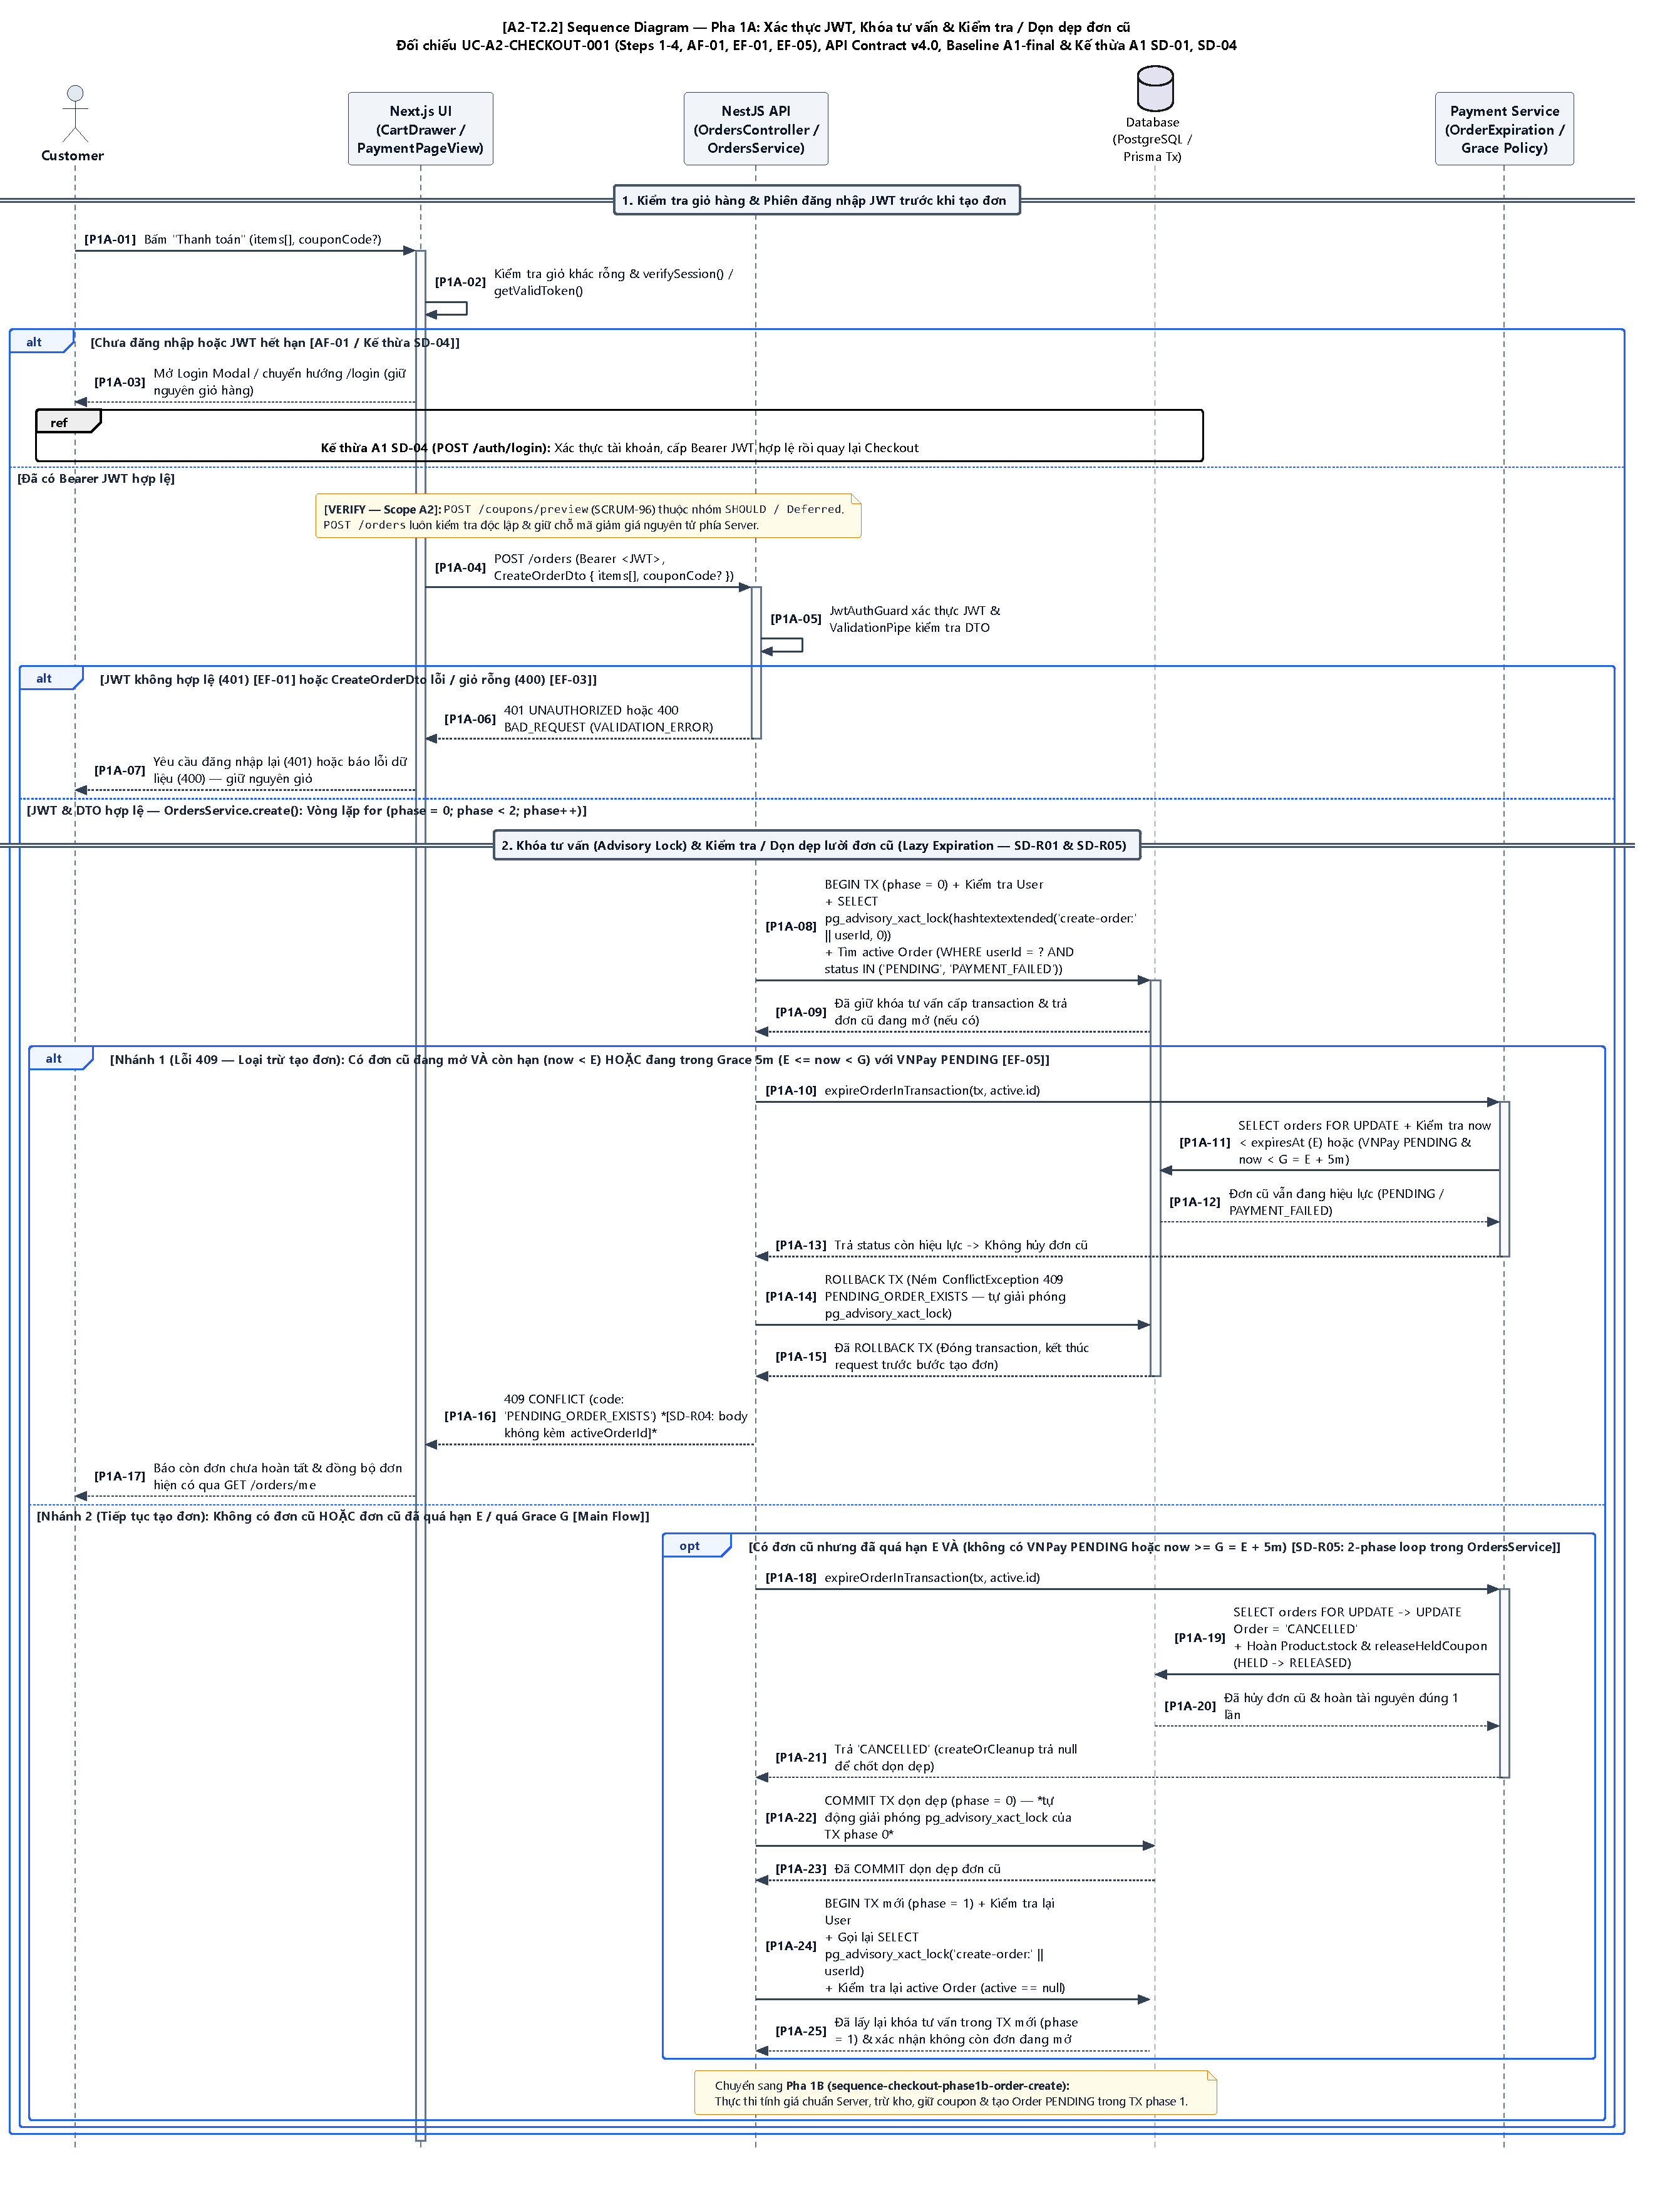
\includegraphics[width=0.95\linewidth,height=0.72\textheight,keepaspectratio]{../assets/sequence-checkout-phase1a-order-init.pdf}%
    }{%
      \fbox{\parbox{0.85\linewidth}{\centering Sơ đồ Pha 1A nằm tại \texttt{docs/report/assets/sequence-checkout-phase1a-order-init.pdf}.}}%
    }%
  }
  \caption[Sequence: xác thực và khởi tạo Order]{Sequence Diagram Pha 1A — Xác thực JWT, khối \texttt{alt} loại trừ \texttt{409} và vòng đời khóa tư vấn qua 2 pha dọn dẹp.}
  \label{fig:seq-phase1a}
\end{figure}

\subsection{Pha 1B: Giao dịch Tạo đơn hàng Nguyên tử (Tính giá, Khóa kho, Giữ Coupon \& Tạo Order)}

Hình~\ref{fig:seq-phase1b} biểu diễn nửa sau Pha 1 trong Transaction sạch (\texttt{phase = 1}): tính giá phía server (\texttt{priceCart}), trừ giữ chỗ tồn kho (\texttt{reserveInventory}), giữ chỗ coupon (\texttt{reserveCoupon HELD}) và tạo bản ghi \texttt{Order (status = 'PENDING', expiresAt = E = now + 15m)} cùng các bản chụp \texttt{OrderItem} / \texttt{OrderItemTopping}. Mọi nhánh lỗi đều \texttt{ROLLBACK TX} và đóng lifeline tường minh.

\begin{figure}[htbp]
  \centering
  \IfFileExists{\BrewLiteSeqDiagramDir/sequence-checkout-phase1b-order-create.pdf}{%
    \includegraphics[width=0.92\linewidth,height=0.68\textheight,keepaspectratio]{\BrewLiteSeqDiagramDir/sequence-checkout-phase1b-order-create.pdf}%
  }{%
    \IfFileExists{../assets/sequence-checkout-phase1b-order-create.pdf}{%
      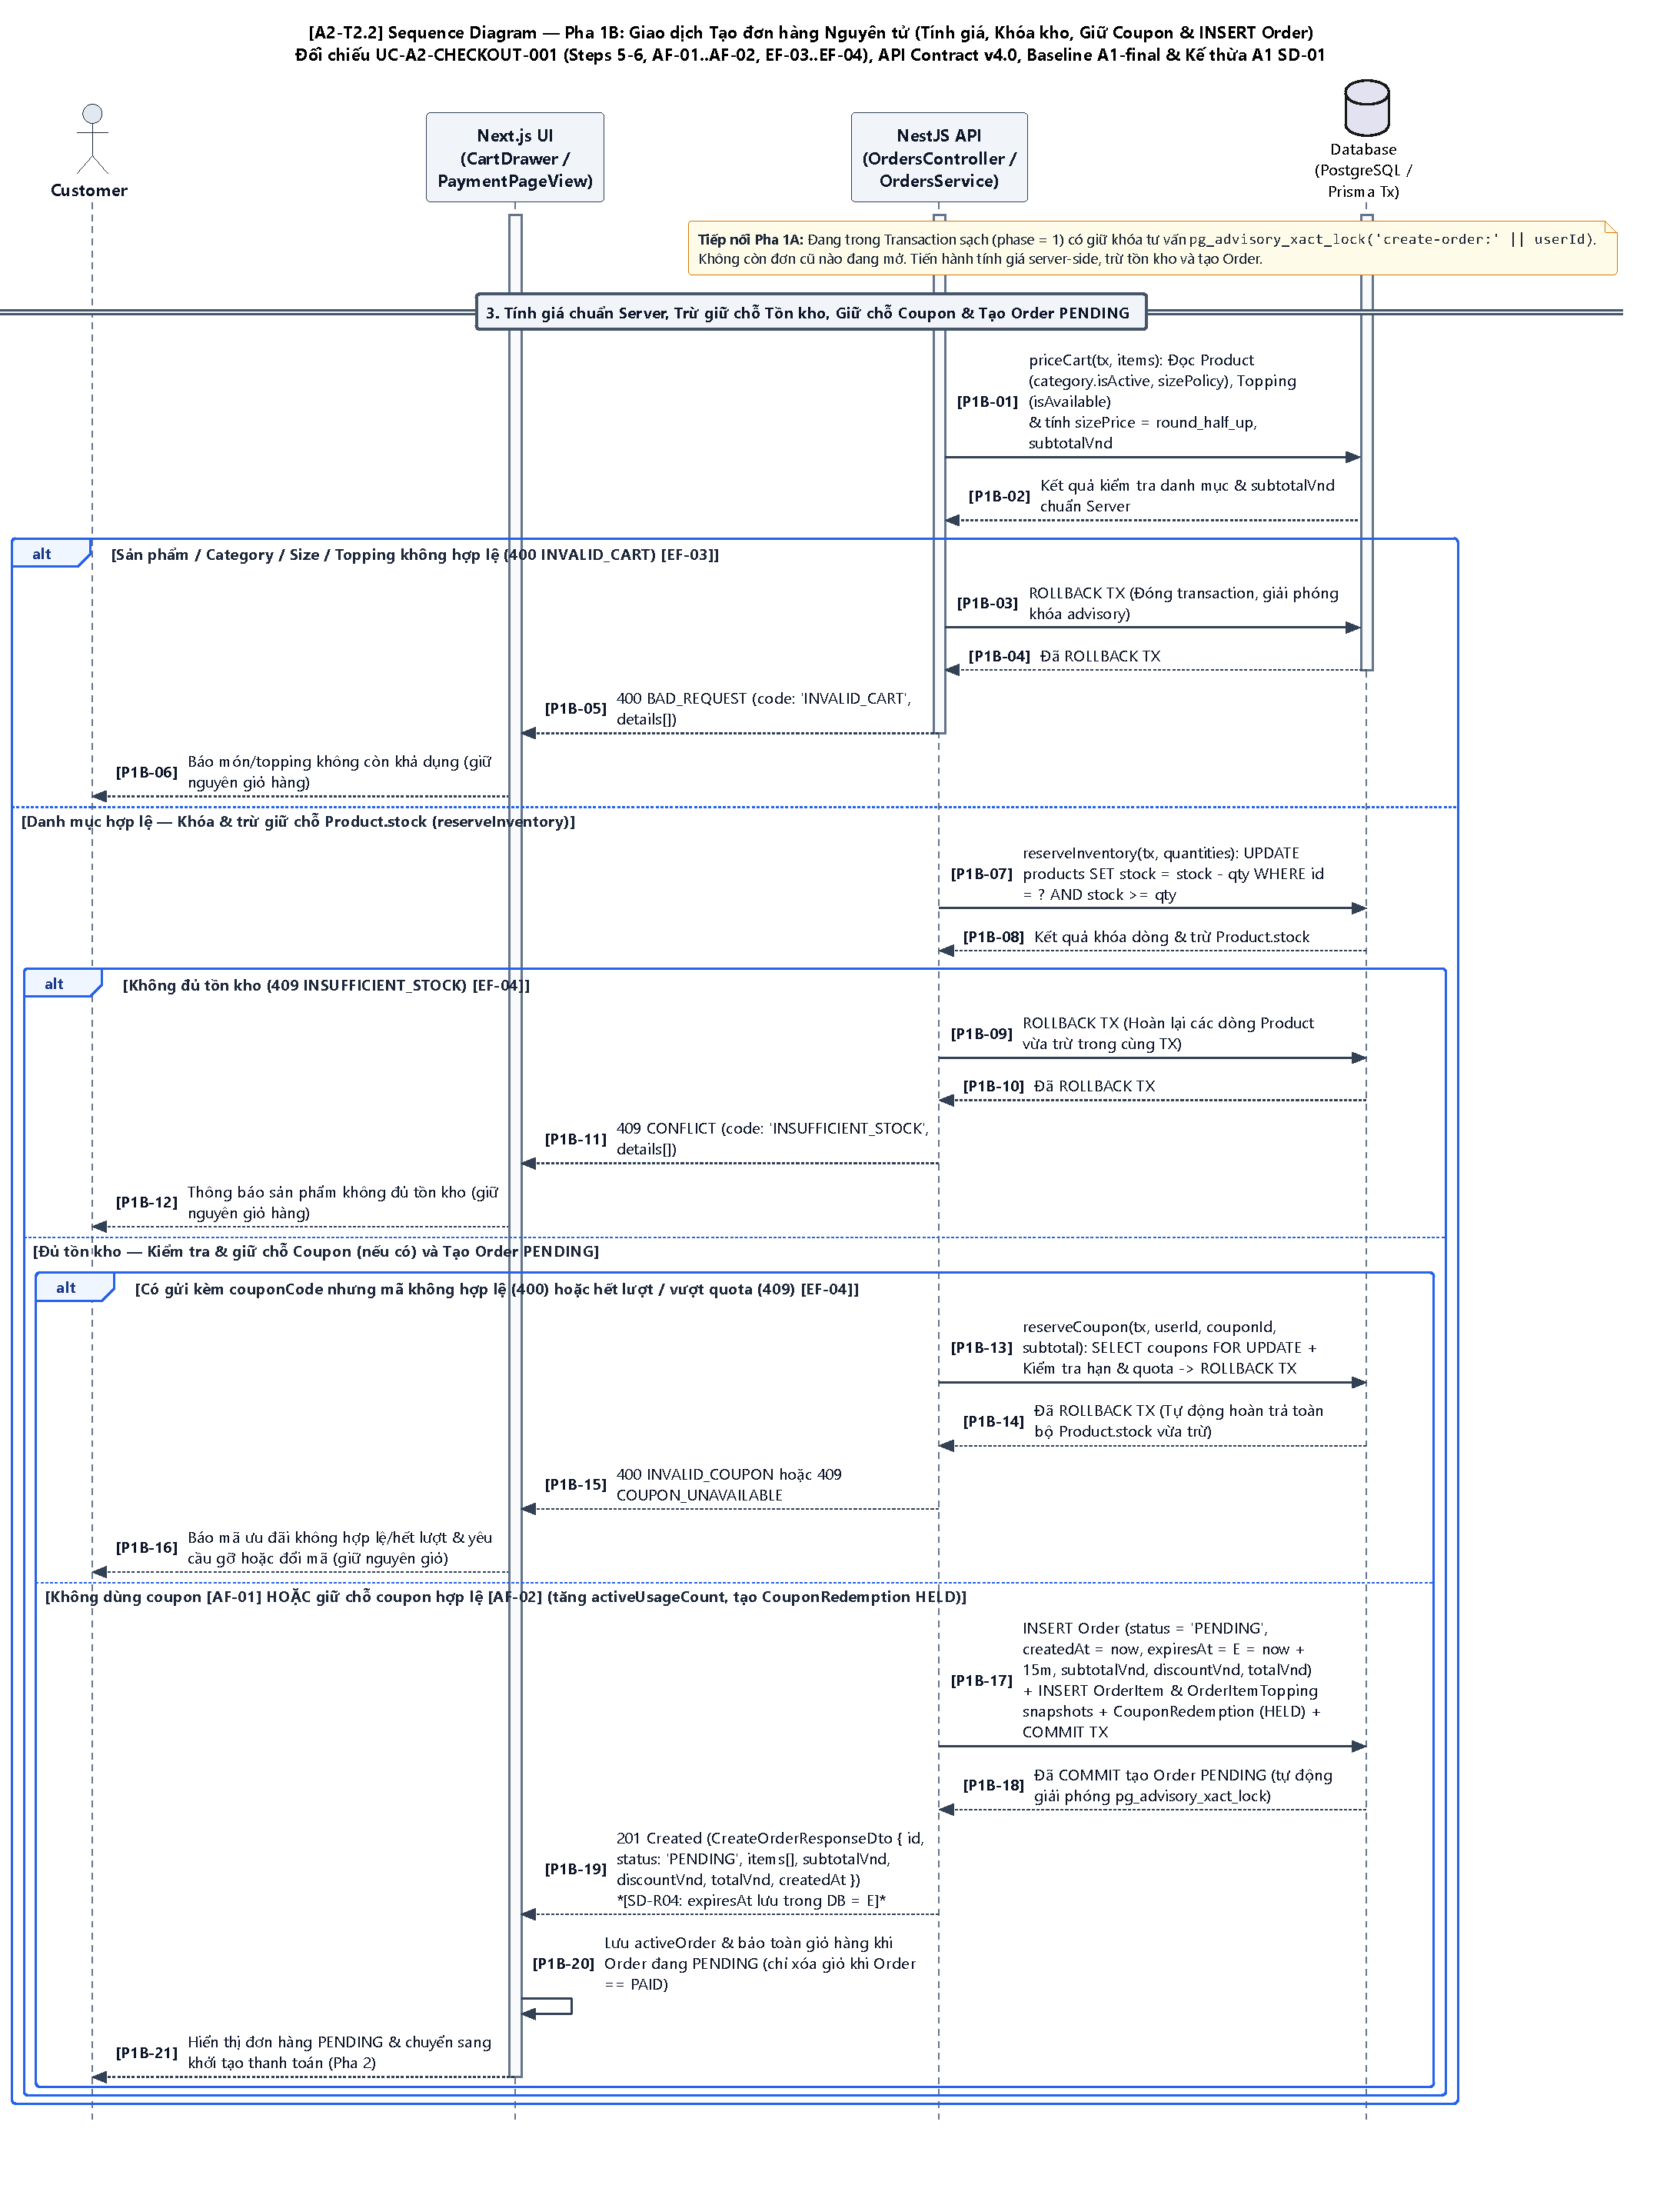
\includegraphics[width=0.92\linewidth,height=0.68\textheight,keepaspectratio]{../assets/sequence-checkout-phase1b-order-create.pdf}%
    }{%
      \fbox{\parbox{0.85\linewidth}{\centering Sơ đồ Pha 1B nằm tại \texttt{docs/report/assets/sequence-checkout-phase1b-order-create.pdf}.}}%
    }%
  }
  \caption[Sequence: transaction tạo Order]{Sequence Diagram Pha 1B — Giao dịch tạo đơn hàng nguyên tử: tính giá chuẩn server, khóa kho, giữ coupon và tạo \texttt{Order PENDING}.}
  \label{fig:seq-phase1b}
\end{figure}

\subsection{Pha 2A: Giao thức Idempotency, Kiểm tra Quyền sở hữu \& Khóa tư vấn Thanh toán}

Hình~\ref{fig:seq-phase2a} mô tả giao thức kiểm soát \texttt{Idempotency-Key} thống nhất: kiểm tra quyền sở hữu (\texttt{404 NOT\_FOUND}), tra cứu \texttt{(userId, idempotencyKey)} cùng mã băm \texttt{requestHash} SHA-256 (\texttt{200 OK} Replay vs \texttt{409 IDEMPOTENCY\_KEY\_CONFLICT}), khóa tư vấn không chặn \texttt{pg\_try\_advisory\_xact\_lock} (\texttt{409 PAYMENT\_IN\_PROGRESS}), khóa dòng \texttt{Order FOR UPDATE} và kiểm tra thời hạn \texttt{now < E}.

\begin{figure}[htbp]
  \centering
  \IfFileExists{\BrewLiteSeqDiagramDir/sequence-checkout-phase2a-idempotency.pdf}{%
    \includegraphics[width=0.95\linewidth,height=0.75\textheight,keepaspectratio]{\BrewLiteSeqDiagramDir/sequence-checkout-phase2a-idempotency.pdf}%
  }{%
    \IfFileExists{../assets/sequence-checkout-phase2a-idempotency.pdf}{%
      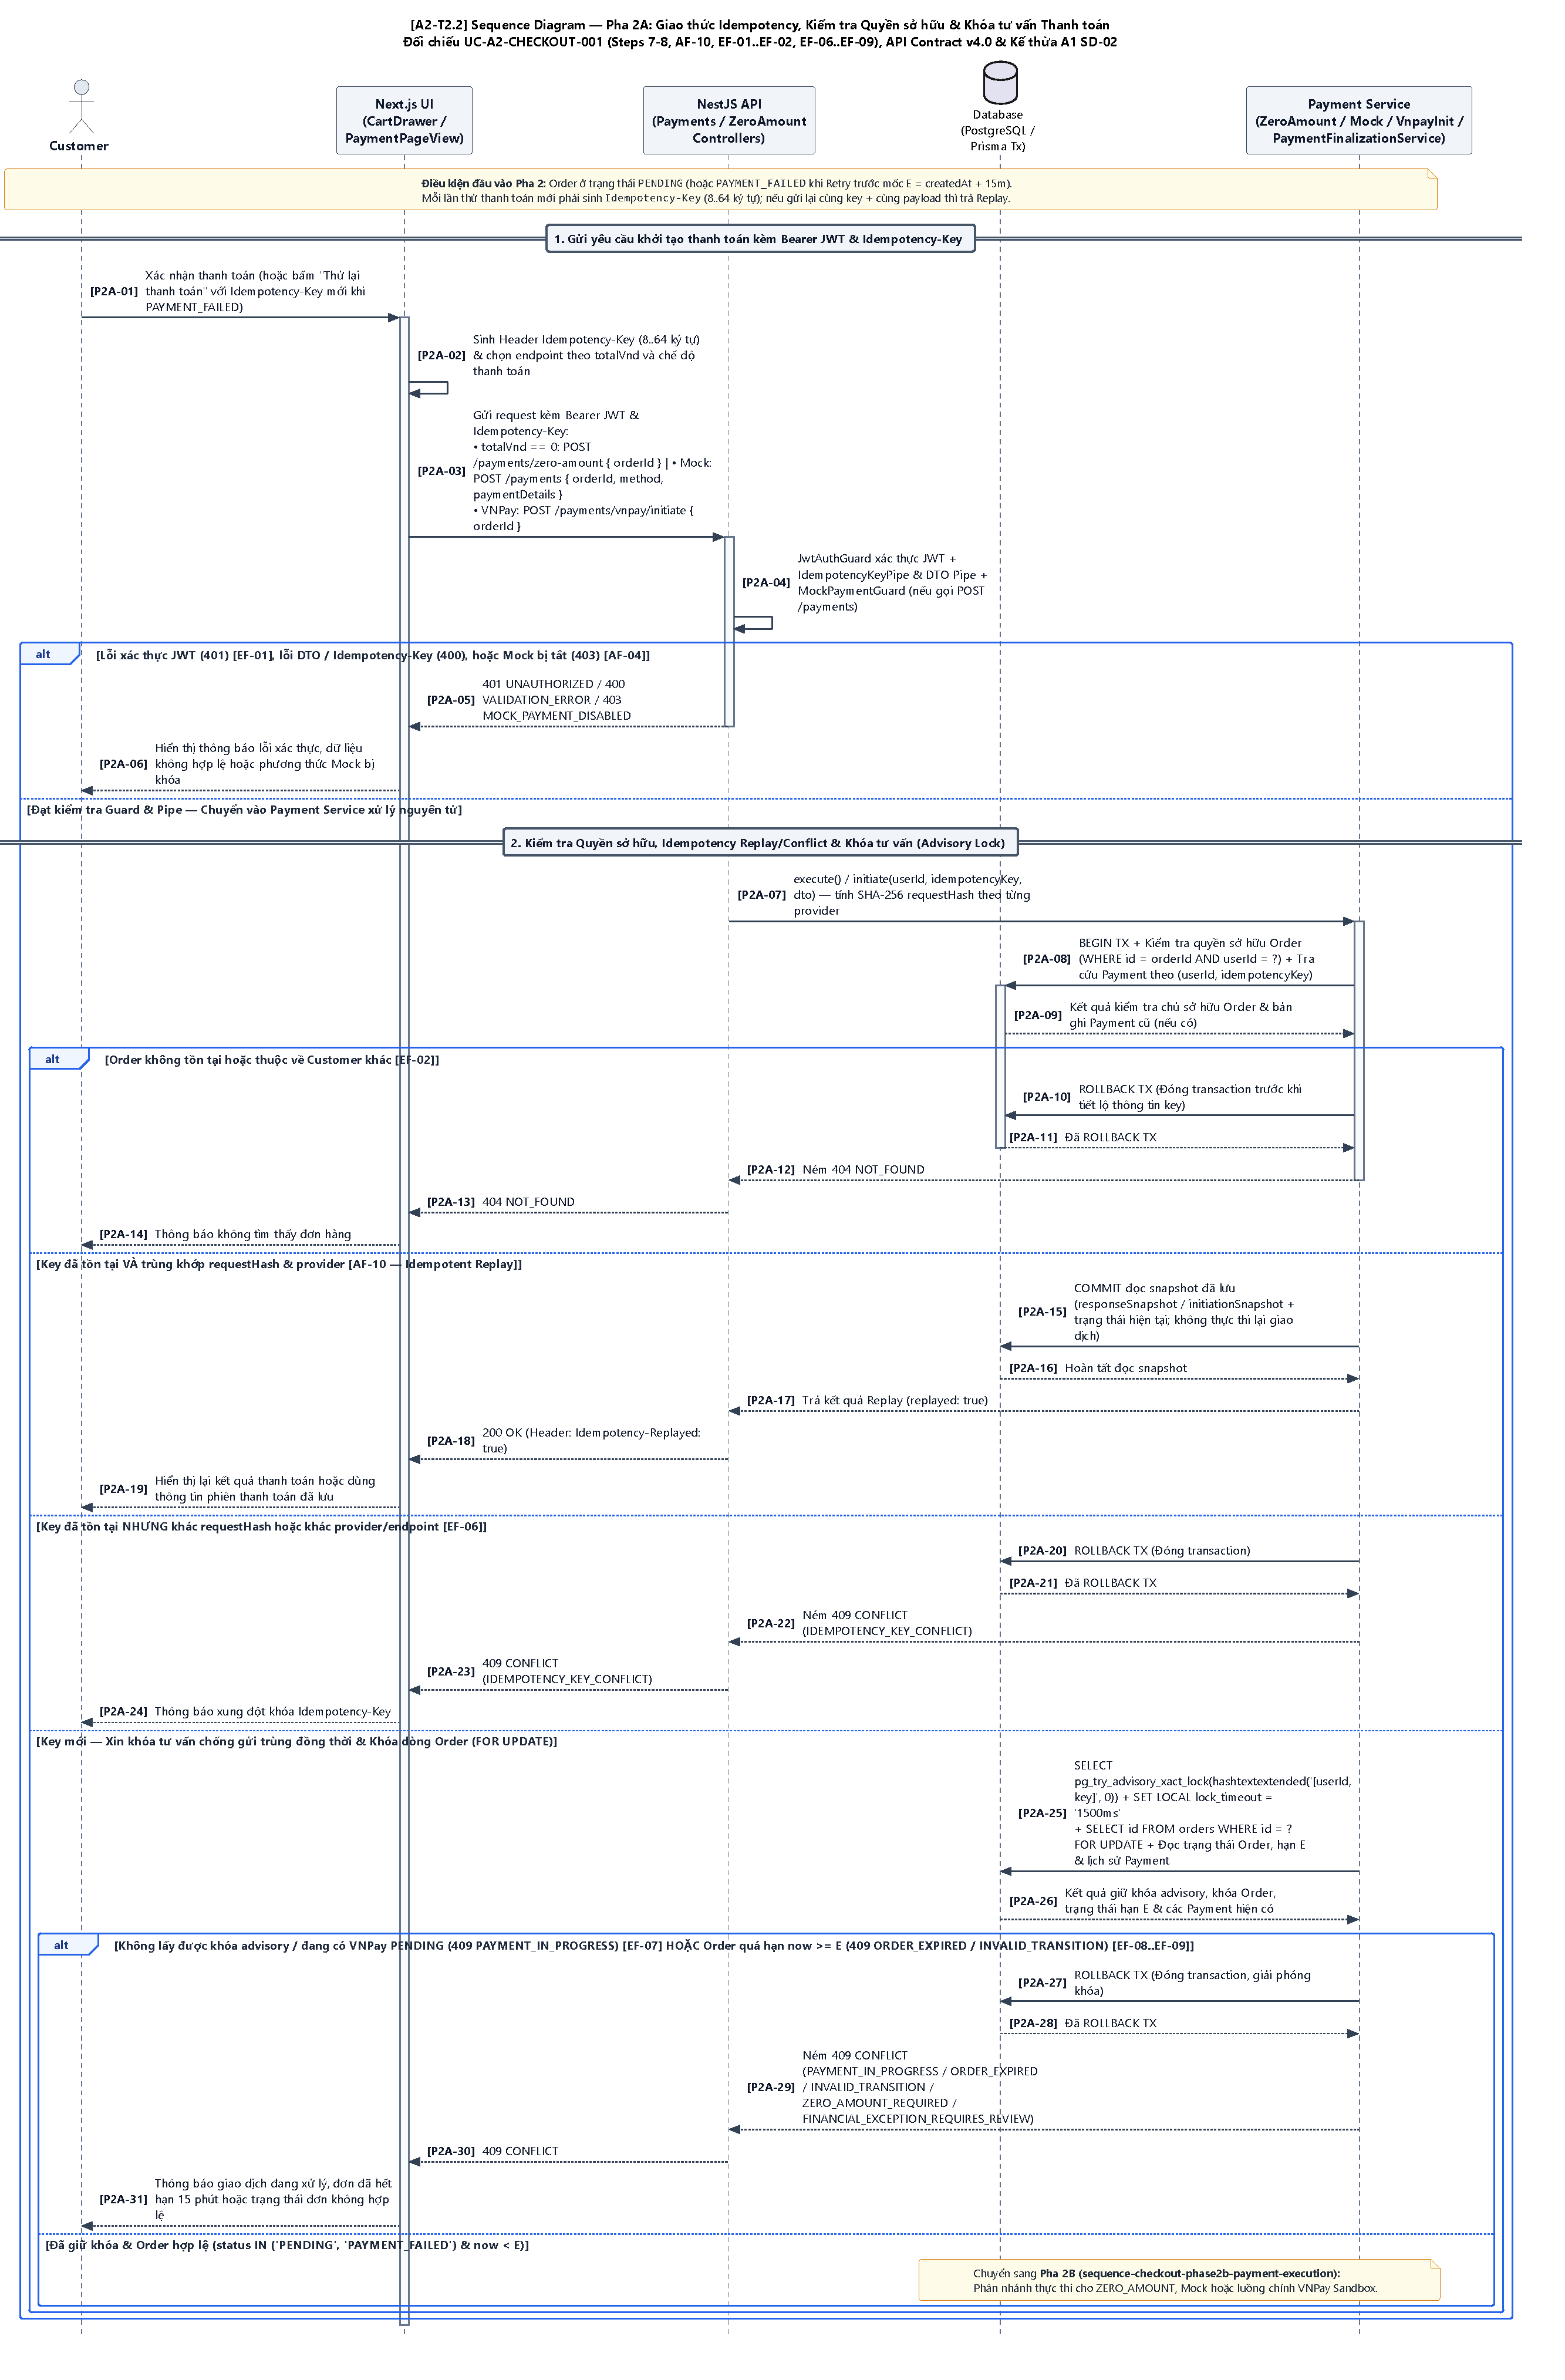
\includegraphics[width=0.95\linewidth,height=0.75\textheight,keepaspectratio]{../assets/sequence-checkout-phase2a-idempotency.pdf}%
    }{%
      \fbox{\parbox{0.85\linewidth}{\centering Sơ đồ Pha 2A nằm tại \texttt{docs/report/assets/sequence-checkout-phase2a-idempotency.pdf}.}}%
    }%
  }
  \caption[Sequence: payment idempotency]{Sequence Diagram Pha 2A — Giao thức Idempotency, kiểm tra quyền sở hữu và khóa tư vấn thanh toán (\texttt{pg\_try\_advisory\_xact\_lock}).}
  \label{fig:seq-phase2a}
\end{figure}

\subsection{Pha 2B: Các nhánh thanh toán (ZERO\_AMOUNT, Mock \& VNPay Initiate)}

Hình~\ref{fig:seq-phase2b} mô tả ba nhánh thực thi thanh toán khi Order và Idempotency-Key hợp lệ:
\begin{itemize}
  \item \textbf{Nhánh A (\texttt{totalVnd == 0}):} \texttt{finalizeInTransaction(provider = 'ZERO\_AMOUNT')} chuyển coupon \texttt{HELD \(\rightarrow\) CONSUMED}, cập nhật \texttt{Order \(\rightarrow\) PAID} (\texttt{pointsEarned = 0}, \texttt{paidAt = clock.now}), lưu \texttt{Payment (ZERO\_AMOUNT, SUCCESS)} và trả \texttt{201 Created}.
  \item \textbf{Nhánh B (\texttt{Mock CARD/WALLET}):} Được bảo vệ bởi \texttt{MockPaymentGuard}. Nếu \texttt{SUCCESS}: coupon \texttt{CONSUMED}, cộng điểm, \texttt{Order \(\rightarrow\) PAID} (\texttt{paidAt = clock.now}). Nếu \texttt{FAILED}: giữ nguyên kho \& coupon \texttt{HELD}, \texttt{Order \(\rightarrow\) PAYMENT\_FAILED} cho phép Retry trước mốc $E$.
  \item \textbf{Nhánh C (\texttt{VNPay Sandbox Initiate}):} Sinh \texttt{paymentId}, \texttt{vnpTxnRef} mới (32-hex), ký \texttt{HMAC-SHA512} tạo \texttt{paymentUrl}, lưu \texttt{Payment PENDING} (\texttt{reconciliationState = SCHEDULED}) và điều hướng trình duyệt sang cổng VNPay.
\end{itemize}

\begin{figure}[htbp]
  \centering
  \IfFileExists{\BrewLiteSeqDiagramDir/sequence-checkout-phase2b-payment-execution.pdf}{%
    \includegraphics[width=0.92\linewidth,height=0.68\textheight,keepaspectratio]{\BrewLiteSeqDiagramDir/sequence-checkout-phase2b-payment-execution.pdf}%
  }{%
    \IfFileExists{../assets/sequence-checkout-phase2b-payment-execution.pdf}{%
      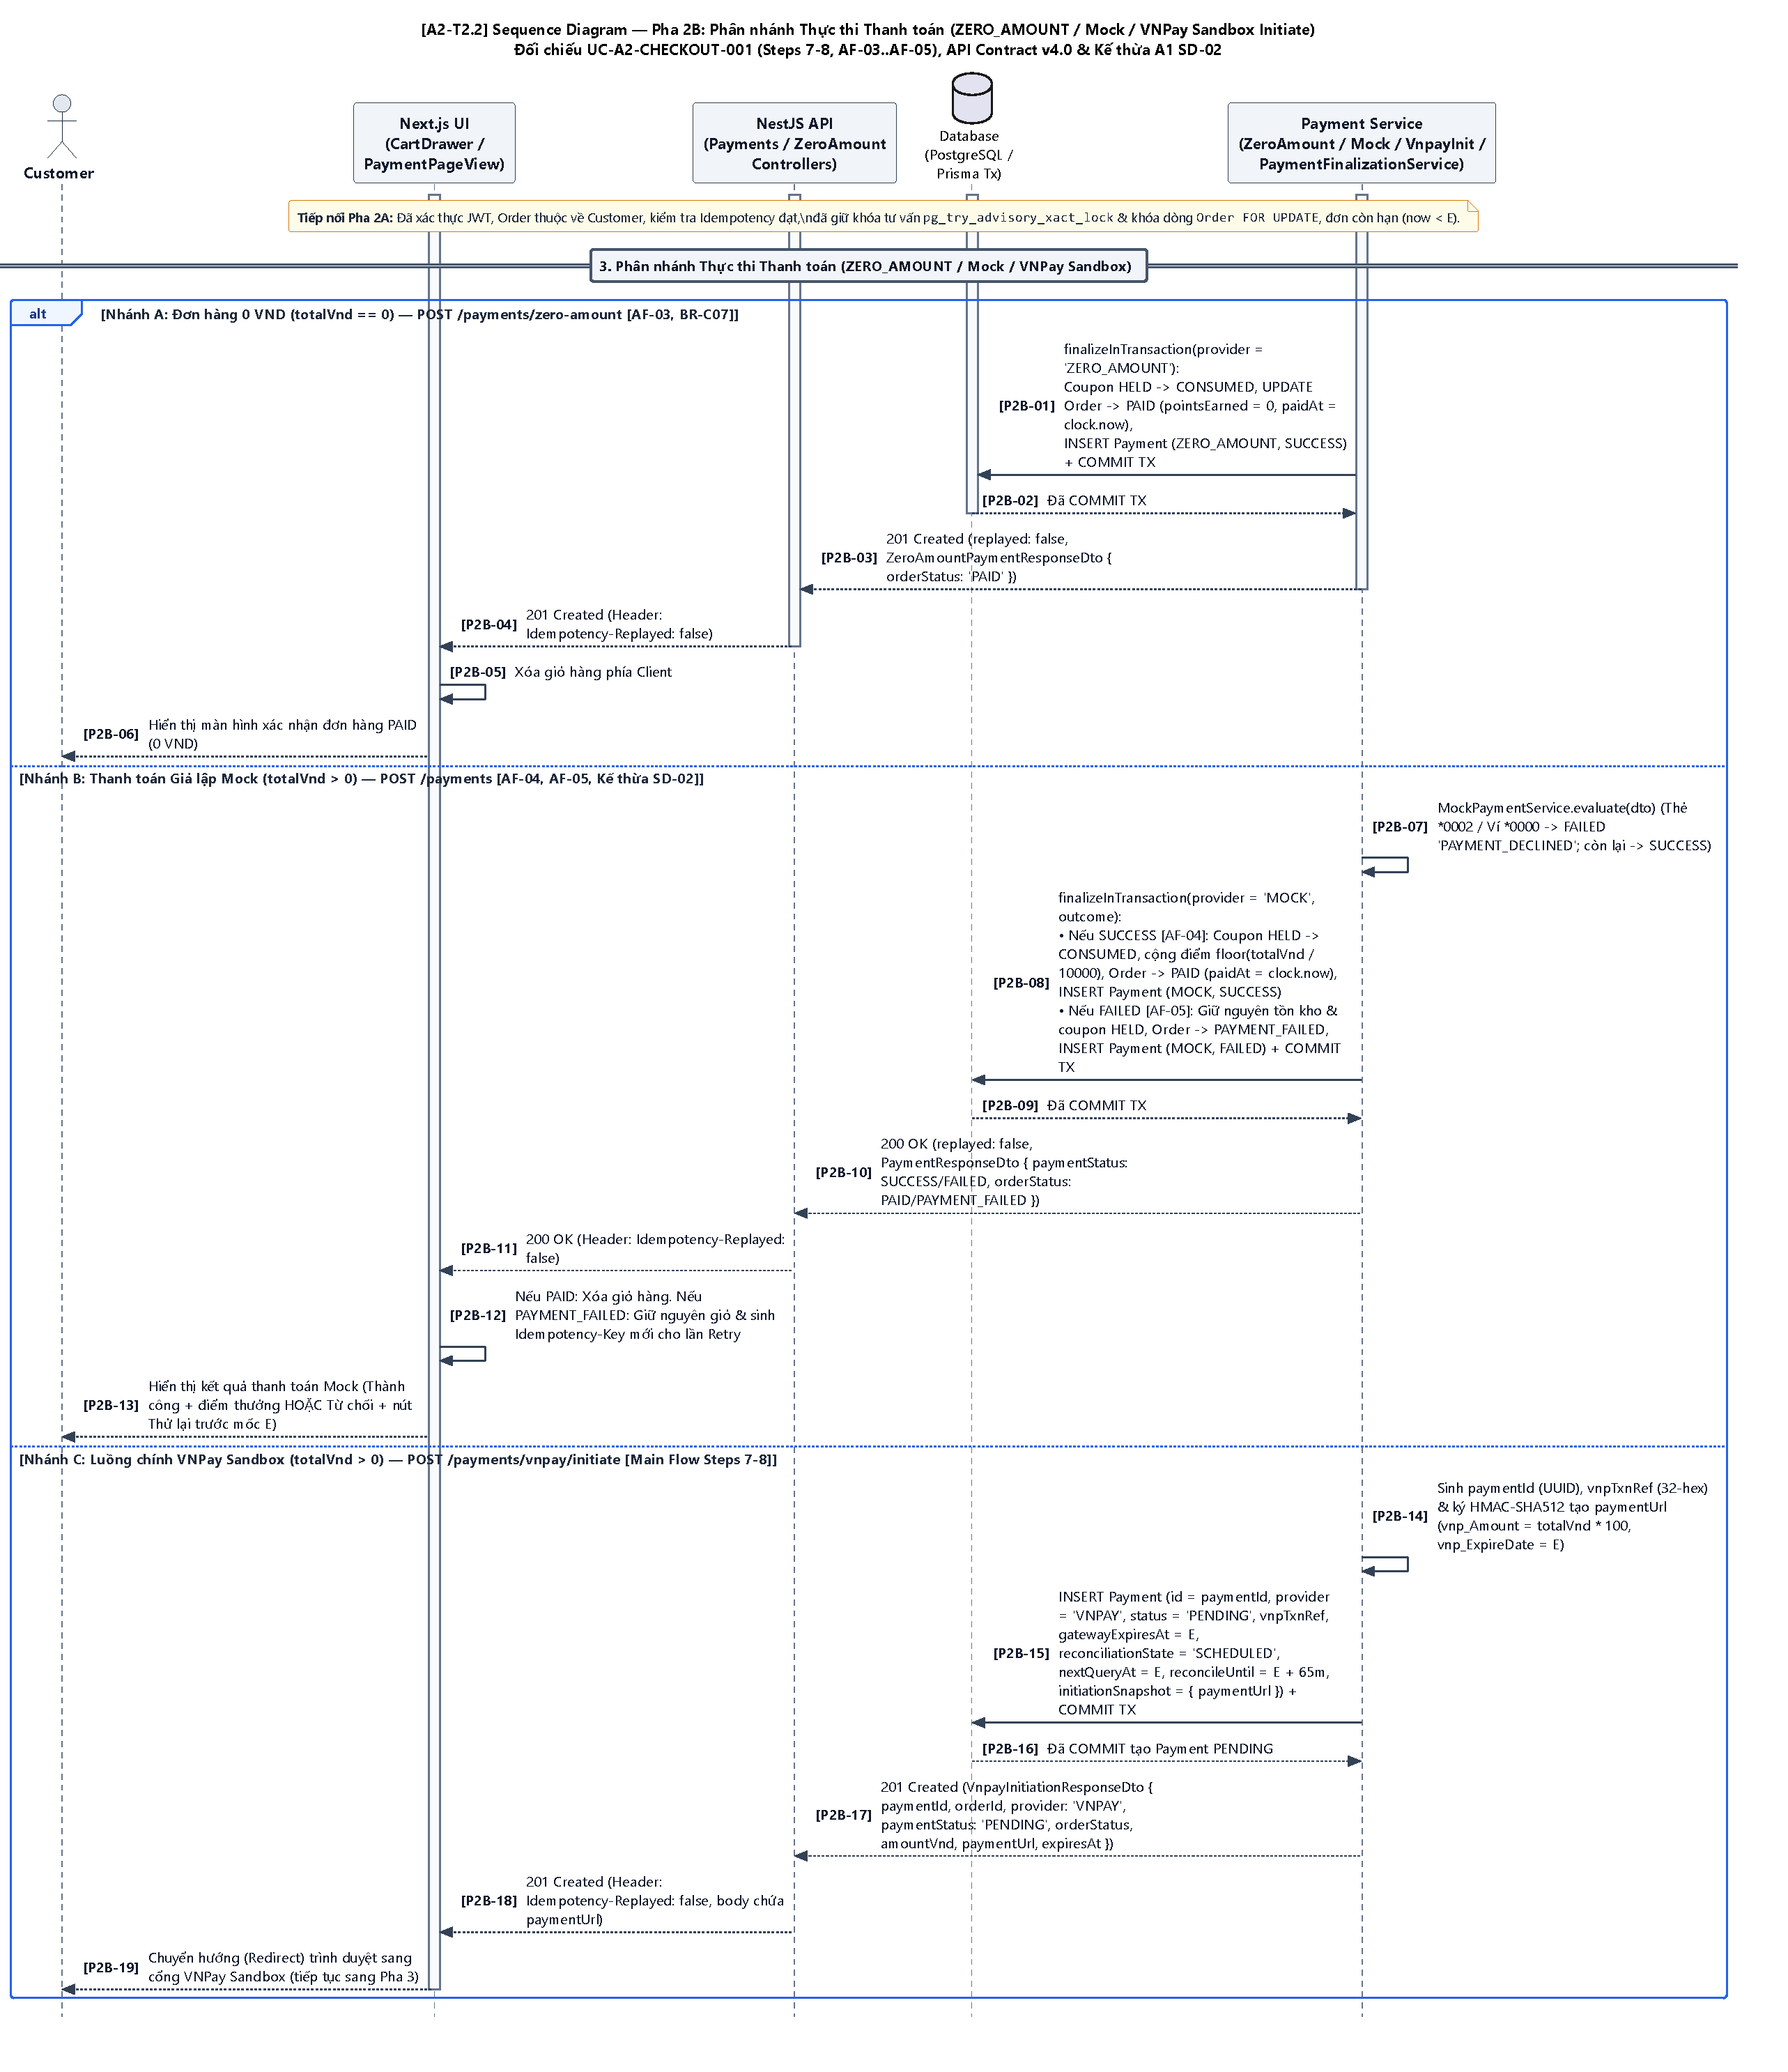
\includegraphics[width=0.92\linewidth,height=0.68\textheight,keepaspectratio]{../assets/sequence-checkout-phase2b-payment-execution.pdf}%
    }{%
      \fbox{\parbox{0.85\linewidth}{\centering Sơ đồ Pha 2B nằm tại \texttt{docs/report/assets/sequence-checkout-phase2b-payment-execution.pdf}.}}%
    }%
  }
  \caption[Sequence: các nhánh payment]{Sequence Diagram Pha 2B — Phân nhánh thực thi: đơn \texttt{0 VND}, giả lập \texttt{Mock} và khởi tạo thanh toán \texttt{VNPay Sandbox}.}
  \label{fig:seq-phase2b}
\end{figure}

\subsection{Pha 3A: Xử lý Webhook Server-to-Server IPN \& Chốt giao dịch (Shared Finalization)}

Hình~\ref{fig:seq-phase3a} biểu diễn luồng IPN độc lập ở phía Server (nguồn sự thật chốt kết quả tại Backend):
\begin{enumerate}
  \item Kiểm tra chữ ký số \texttt{HMAC-SHA512} và \texttt{vnp\_TmnCode}; nếu lỗi trả \texttt{RspCode 97/99} mà \textbf{không mở DB transaction}.
  \item Mở transaction kiểm tra \texttt{vnpTxnRef} và số tiền (\texttt{vnp\_Amount == amountVnd * 100}); nếu lỗi trả \texttt{RspCode 01/04} và đóng transaction không sửa dữ liệu.
  \item Khóa chuẩn \texttt{Order FOR UPDATE} $\rightarrow$ \texttt{Payment FOR UPDATE} (\texttt{EF-13, BR-C05}) và đối chiếu thời điểm thanh toán \texttt{gatewayPaidAt} (\texttt{vnp\_PayDate}) với thời điểm DB finalization \texttt{clock.now}:
  \begin{itemize}
    \item \emph{Thành công đúng hạn (\texttt{gatewayPaidAt <= E} \& \texttt{clock.now < G}):} Cập nhật \texttt{Payment \(\rightarrow\) SUCCESS} (\texttt{verifiedPaidAt = gatewayPaidAt}, \texttt{finalizedAt = clock.now}) và \texttt{Order \(\rightarrow\) PAID} (\texttt{paidAt = clock.now}).
    \item \emph{Thành công đến trễ / Xung đột (\texttt{gatewayPaidAt > E} hoặc \texttt{clock.now >= G}):} Ghi nhận \texttt{FINANCIAL\_EXCEPTION}, giữ nguyên \texttt{Payment.status}, đặt \texttt{reconciliationState = REQUIRES\_REVIEW} và hủy \texttt{Order \(\rightarrow\) CANCELLED} nếu đang mở (không hồi sinh sang \texttt{PAID}).
    \item \emph{Thất bại terminal:} Cập nhật \texttt{Payment \(\rightarrow\) FAILED}; nếu \texttt{clock.now < E} thì \texttt{Order \(\rightarrow\) PAYMENT\_FAILED} (cho phép Retry); nếu \texttt{clock.now >= E} thì hủy \texttt{Order \(\rightarrow\) CANCELLED} và hoàn tài nguyên đúng 1 lần.
  \end{itemize}
\end{enumerate}

\begin{figure}[htbp]
  \centering
  \IfFileExists{\BrewLiteSeqDiagramDir/sequence-checkout-phase3a-vnpay-ipn.pdf}{%
    \includegraphics[width=0.95\linewidth,height=0.76\textheight,keepaspectratio]{\BrewLiteSeqDiagramDir/sequence-checkout-phase3a-vnpay-ipn.pdf}%
  }{%
    \IfFileExists{../assets/sequence-checkout-phase3a-vnpay-ipn.pdf}{%
      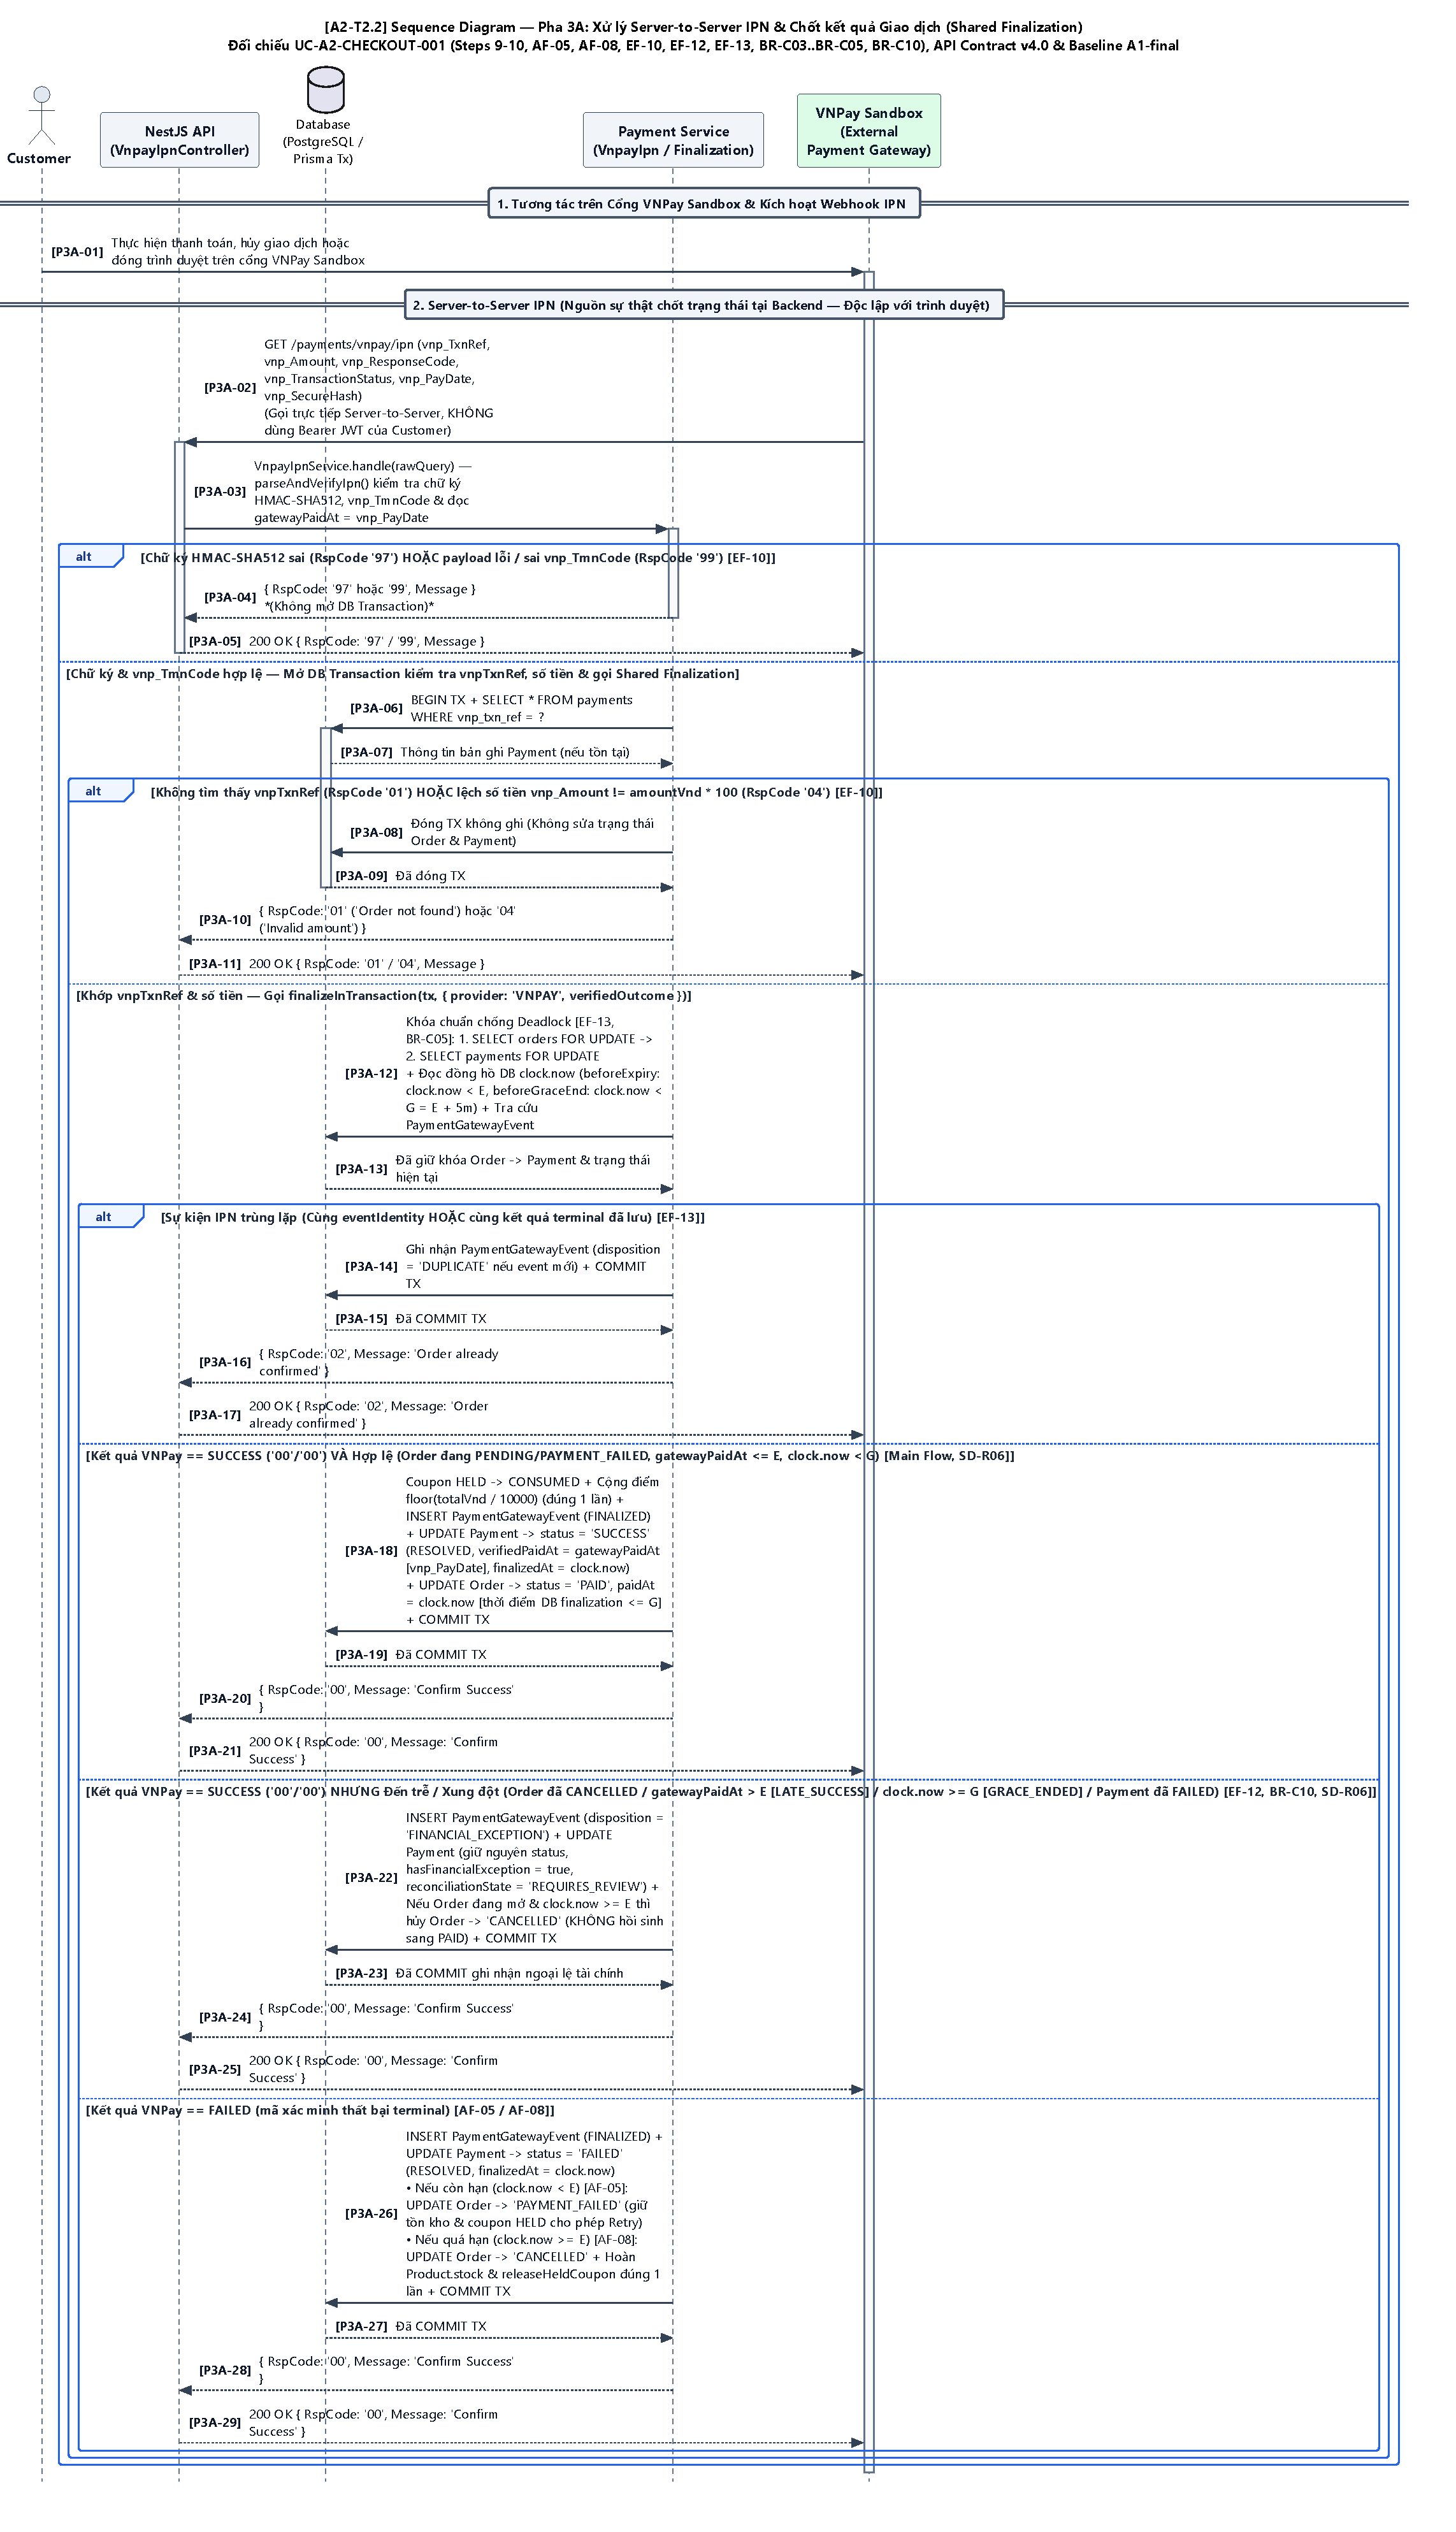
\includegraphics[width=0.95\linewidth,height=0.76\textheight,keepaspectratio]{../assets/sequence-checkout-phase3a-vnpay-ipn.pdf}%
    }{%
      \fbox{\parbox{0.85\linewidth}{\centering Sơ đồ Pha 3A nằm tại \texttt{docs/report/assets/sequence-checkout-phase3a-vnpay-ipn.pdf}.}}%
    }%
  }
  \caption[Sequence: VNPay IPN]{Sequence Diagram Pha 3A — Xử lý Server-to-Server IPN: kiểm tra chữ ký, phân biệt \texttt{gatewayPaidAt <= E} vs \texttt{clock.now < G} và chốt kết quả \texttt{Shared Finalization}.}
  \label{fig:seq-phase3a}
\end{figure}

\subsection{Pha 3B: Browser Return URL, Bounded Polling \& Background Scheduler Đối soát / Hết hạn}

Hình~\ref{fig:seq-phase3b} biểu diễn hai luồng độc lập còn lại của Pha 3:
\begin{itemize}
  \item \textbf{Luồng Browser Return URL (\texttt{EF-11}):} Chỉ điều hướng UI; không tự coi Return URL là \texttt{PAID}. Frontend thực hiện bounded polling \texttt{GET /orders/me} kết hợp \texttt{GET /auth/me} để đồng bộ trạng thái chuẩn từ cơ sở dữ liệu.
  \item \textbf{Luồng Background Scheduler (Mô hình 3 Transaction của \texttt{VnpayQueryDrService}):}
  \begin{itemize}
    \item \textbf{TX 1 (\texttt{claim}):} Khóa \texttt{Order} $\rightarrow$ \texttt{Payment}; nếu \texttt{clock.now >= G} thì hủy đơn sang \texttt{CANCELLED} và giải phóng kho/coupon; cấp \texttt{claimToken} rồi \texttt{COMMIT} để giải phóng khóa DB.
    \item \textbf{HTTP Call:} Gọi \texttt{POST /merchant\_webapi/api/transaction} (\texttt{querydr}) ngoài DB transaction (\texttt{ADR-P2-QueryDR-Sandbox-E2E-Deferred}).
    \item \textbf{TX 2 (\texttt{finalizeInTransaction})} + \textbf{TX 3 (\texttt{releaseClaim})}: Khóa lại và chốt kết quả đối soát, sau đó giải phóng lease. Khi chạm chân trời $H = E + 65\text{m}$, \texttt{markExhausted()} đặt \texttt{reconciliationState = 'REQUIRES\_REVIEW'}.
  \end{itemize}
\end{itemize}

\begin{figure}[htbp]
  \centering
  \IfFileExists{\BrewLiteSeqDiagramDir/sequence-checkout-phase3b-return-scheduler.pdf}{%
    \includegraphics[width=0.95\linewidth,height=0.74\textheight,keepaspectratio]{\BrewLiteSeqDiagramDir/sequence-checkout-phase3b-return-scheduler.pdf}%
  }{%
    \IfFileExists{../assets/sequence-checkout-phase3b-return-scheduler.pdf}{%
      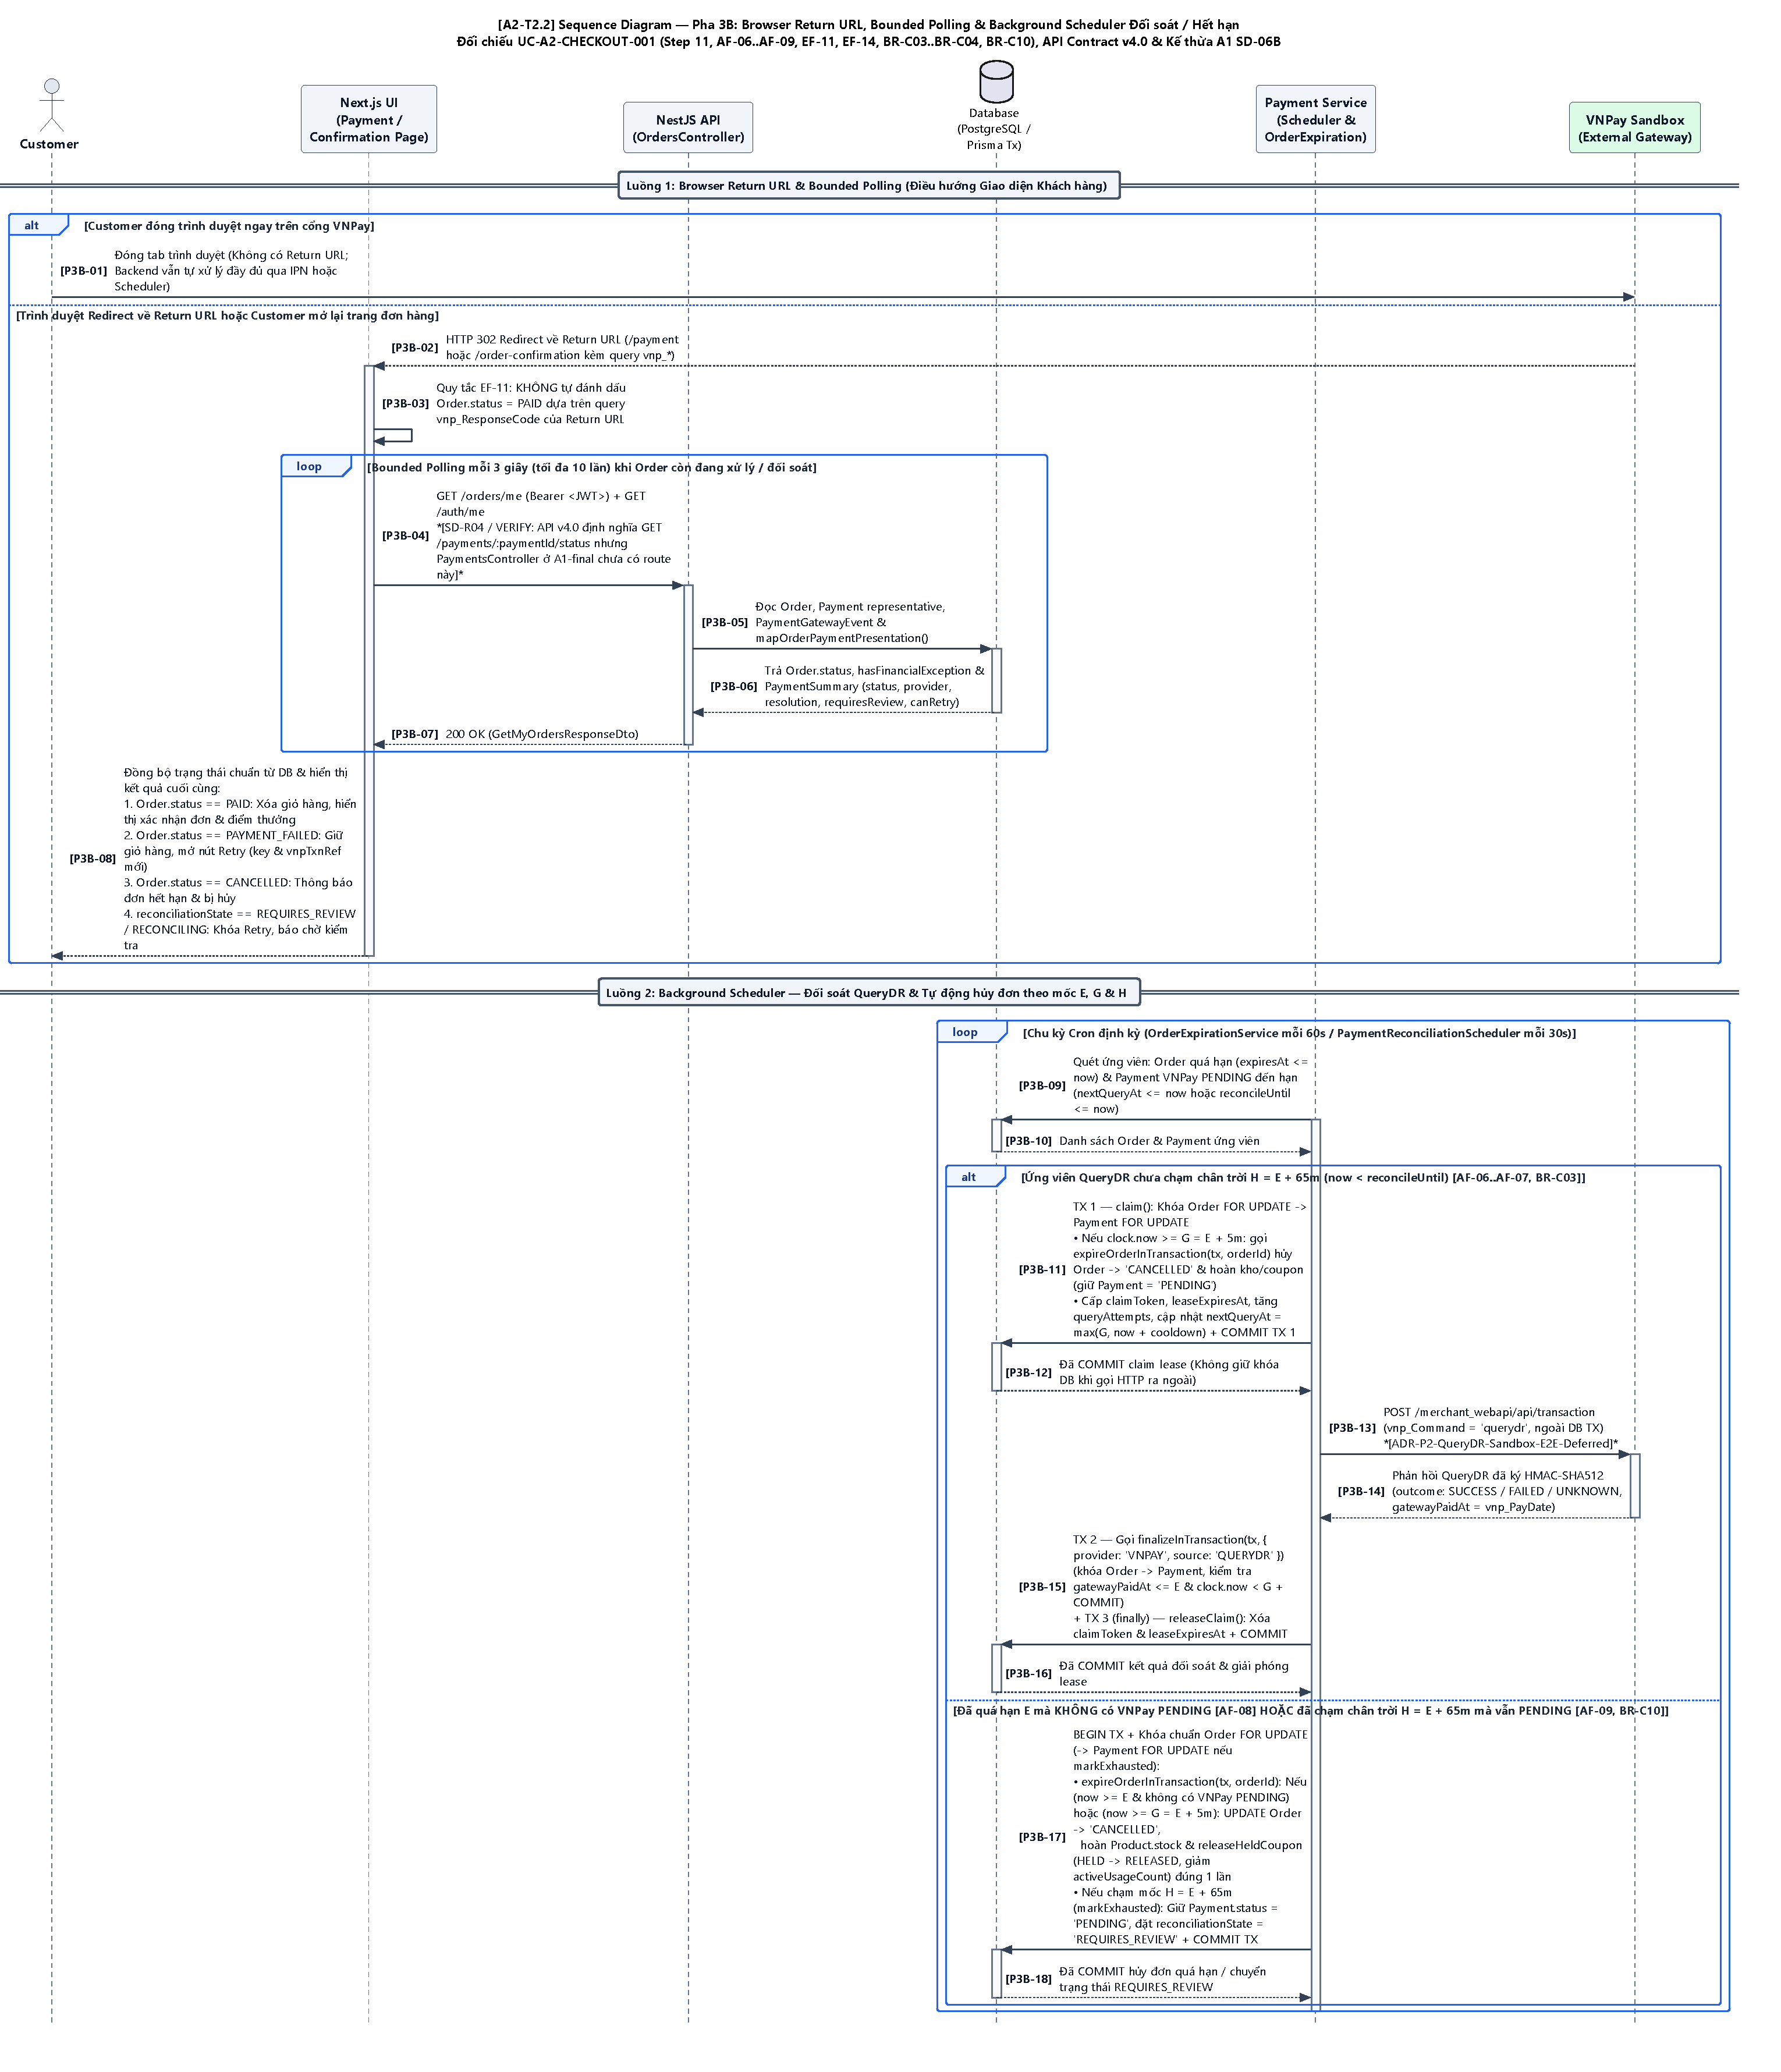
\includegraphics[width=0.95\linewidth,height=0.74\textheight,keepaspectratio]{../assets/sequence-checkout-phase3b-return-scheduler.pdf}%
    }{%
      \fbox{\parbox{0.85\linewidth}{\centering Sơ đồ Pha 3B nằm tại \texttt{docs/report/assets/sequence-checkout-phase3b-return-scheduler.pdf}.}}%
    }%
  }
  \caption[Sequence: Return và reconciliation scheduler]{Sequence Diagram Pha 3B — Browser Return URL, bounded polling \texttt{GET /orders/me} và chu kỳ đối soát QueryDR / hết hạn của Background Scheduler.}
  \label{fig:seq-phase3b}
\end{figure}

Gap payment-status và QueryDR Sandbox được giữ ở đặc tả Checkout và
phần kiểm thử; không lấy thiết kế trong hình làm bằng chứng các luồng đã PASS.
Bảng đối chiếu source lịch sử nằm tại phụ lục nguồn.

\subsection{Sơ đồ Tuần tự Tổng thể (End-to-End Checkout \& Payment)}

Để phục vụ tra cứu kiến trúc tổng quan trên một trang duy nhất (bên cạnh 6 sơ đồ con tách pha có độ phóng đại cao ở các Hình~\ref{fig:seq-phase1a}--\ref{fig:seq-phase3b}), Hình~\ref{fig:seq-checkout-overall} bố trí bản vector tổng thể End-to-End 82 thông điệp trên một trang riêng biệt (\texttt{[p]}).

\clearpage
\begin{figure}[p]
  \centering
  \IfFileExists{\BrewLiteSeqDiagramDir/sequence-checkout.pdf}{%
    \includegraphics[width=\linewidth,height=0.92\textheight,keepaspectratio]{\BrewLiteSeqDiagramDir/sequence-checkout.pdf}%
  }{%
    \IfFileExists{../assets/sequence-checkout.pdf}{%
      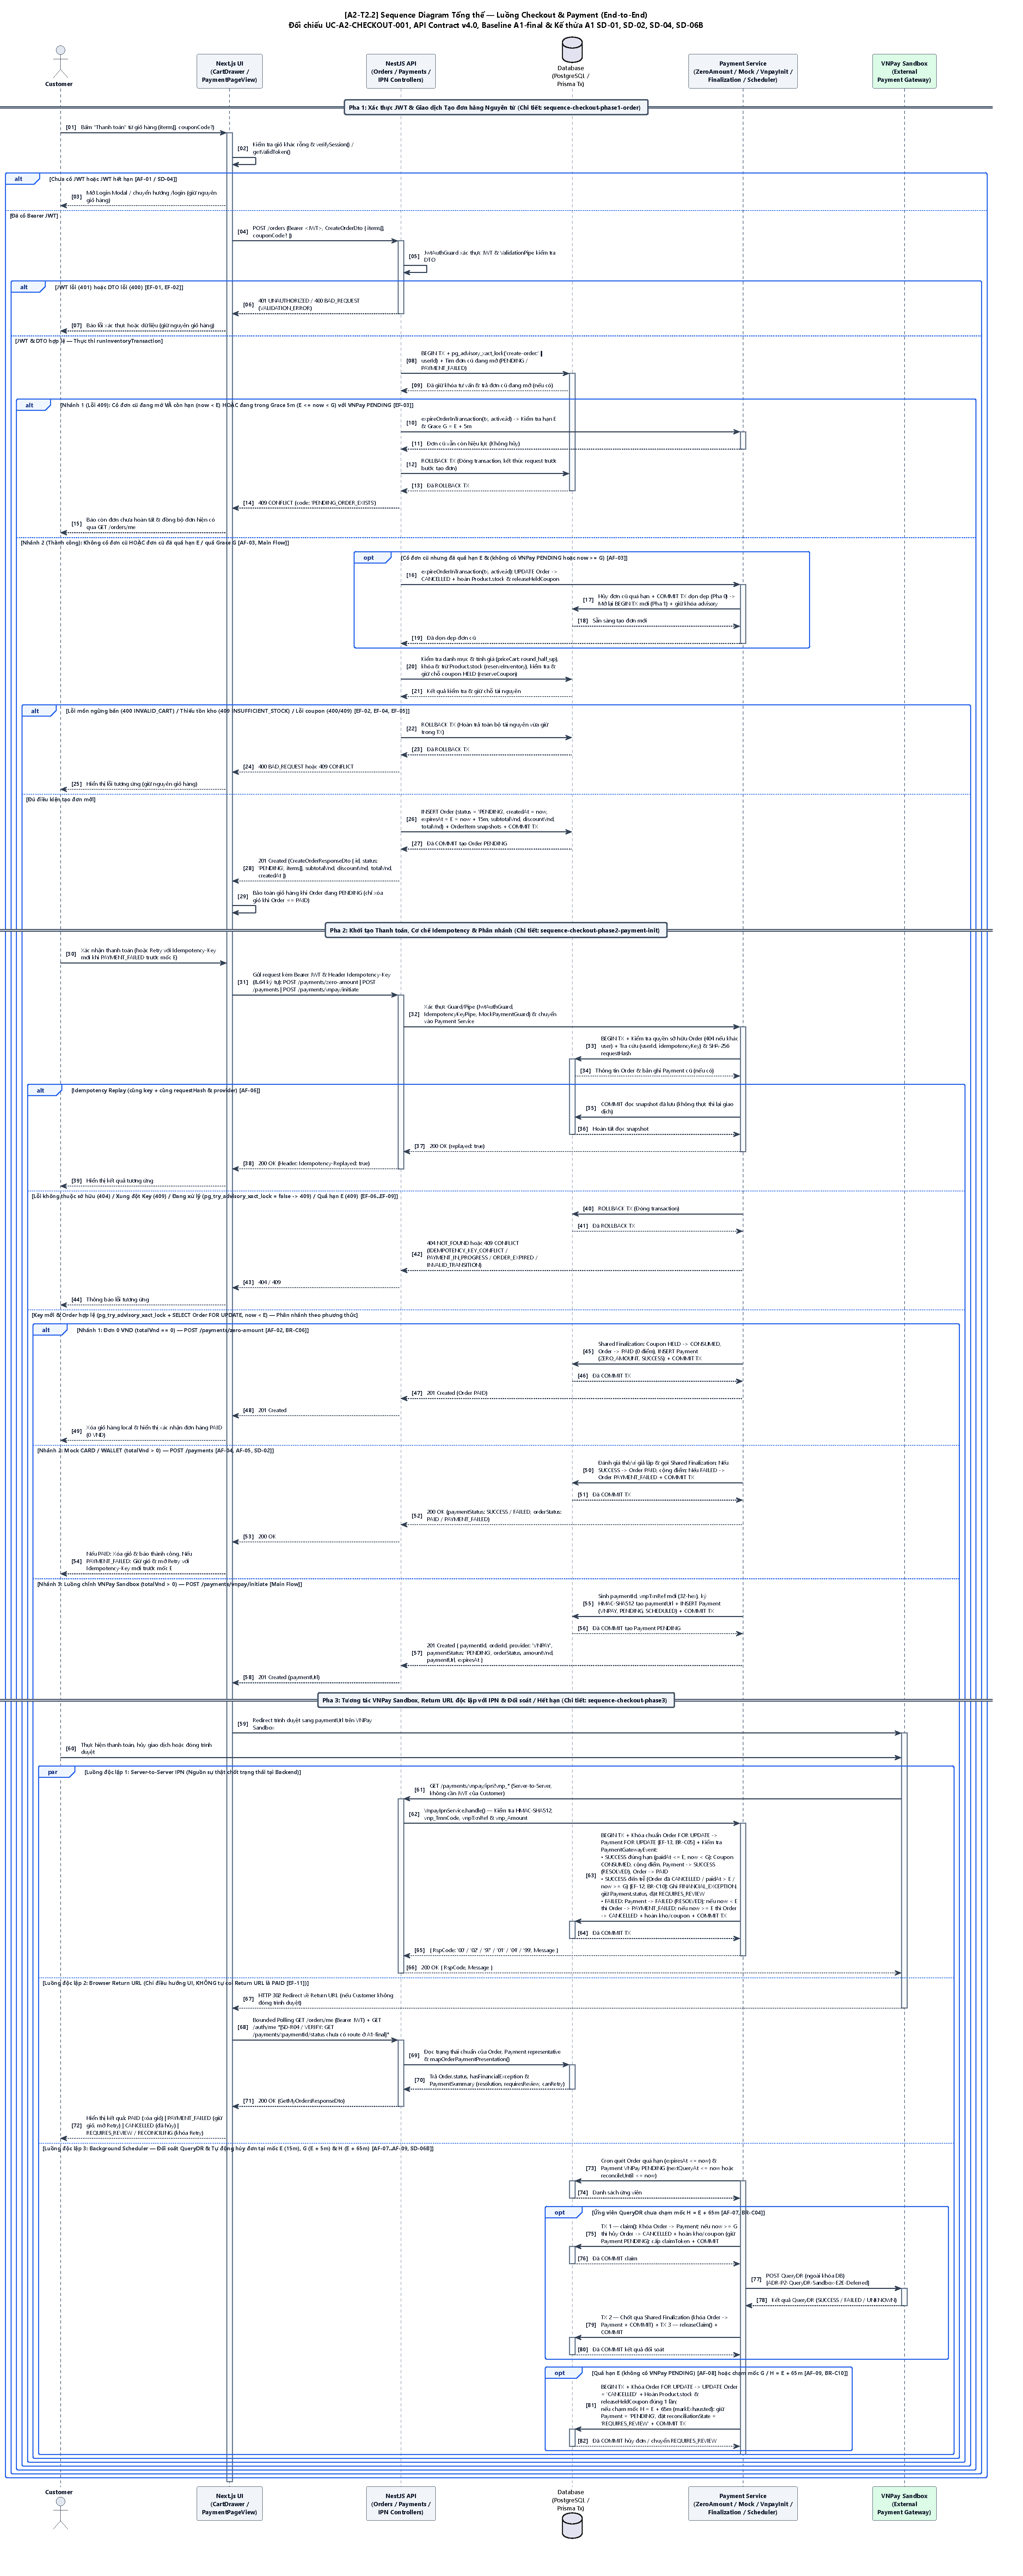
\includegraphics[width=\linewidth,height=0.92\textheight,keepaspectratio]{../assets/sequence-checkout.pdf}%
    }{%
      \fbox{\parbox{0.85\linewidth}{\centering Sơ đồ tổng thể nằm tại \texttt{docs/report/assets/sequence-checkout.pdf}.}}%
    }%
  }
  \caption[Sequence Checkout tổng thể]{Sequence Diagram Tổng thể (End-to-End) — Luồng Checkout \& Payment của BrewLite Assignment 2 (bản vector toàn cảnh đặt trên trang riêng, phục vụ đối chiếu tổng thể kết hợp 6 sơ đồ con độ đọc cao ở Hình~\ref{fig:seq-phase1a}--\ref{fig:seq-phase3b}).}
  \label{fig:seq-checkout-overall}
\end{figure}
\clearpage
